\section{Observando el residuo de predicción}

Para esta parte se utiliza el script \texttt{p5.m}, el cual se adjunta a la entrega

Para lo que sigue de la sección, se considera $e[n]$ como la señal de entrada a filtro AR. Por lo tanto
$$ X(z) = E(z)\cdot H(z)$$
\subsection{Filtro inverso}
Se puede obtener el filtro inverso al AR como el filtro $H(z)^-1$, el cual corresponde a un filtro FIR. A partir de lo anterior se la respuesta en frecuencia del filtro inverso, la cual se muestra en la figura \ref{fig:p5_1}

\begin{figure}[H]
    \centering
    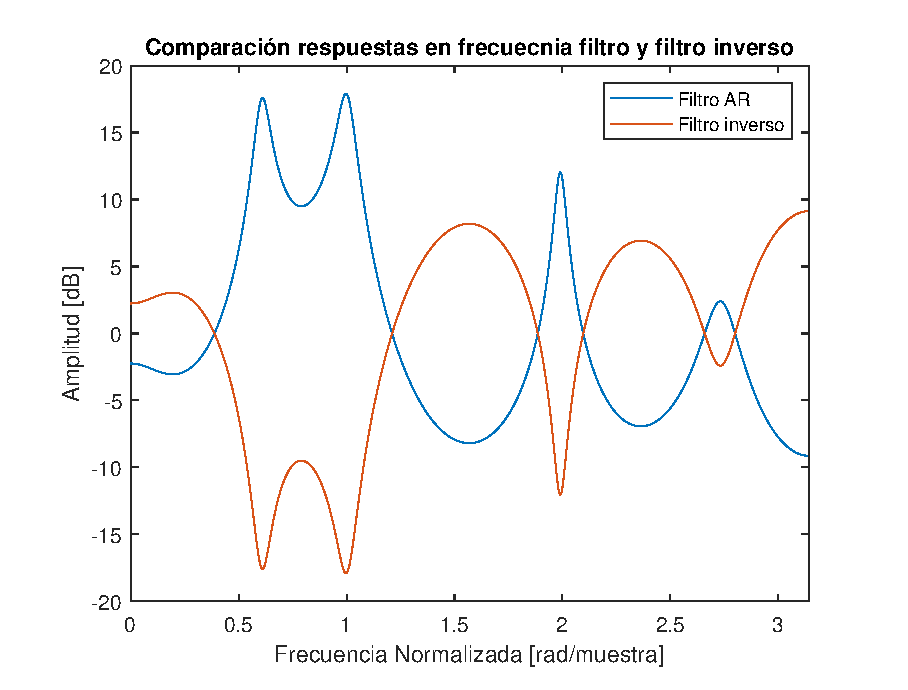
\includegraphics[width = .8\linewidth]{figures/p5_1filtinv.eps}
    \caption{Comparación de respuesta en frecuencia de filtro y filtro inverso.}
    \label{fig:p5_1}
\end{figure}

Como es de esperarse, suma de la respuesta en frecuencia del filtro inverso con el filtro AR es 0.
%%%%%%%%%%%%%%%%%%%%%%%%%%%%%%%%%%%%%%%%%%%%%%%%%%%%%%%%%%%%%%%%%%%%
\subsection{Obtención de la $e[n]$}

Se obtiene $e[n]$ aplicando el filtro inverso a la señal $vowel\_a$. La señal de entrada obtenida se muestra en la figura \ref{fig:p5_2}.

\begin{figure}[H]
    \centering
    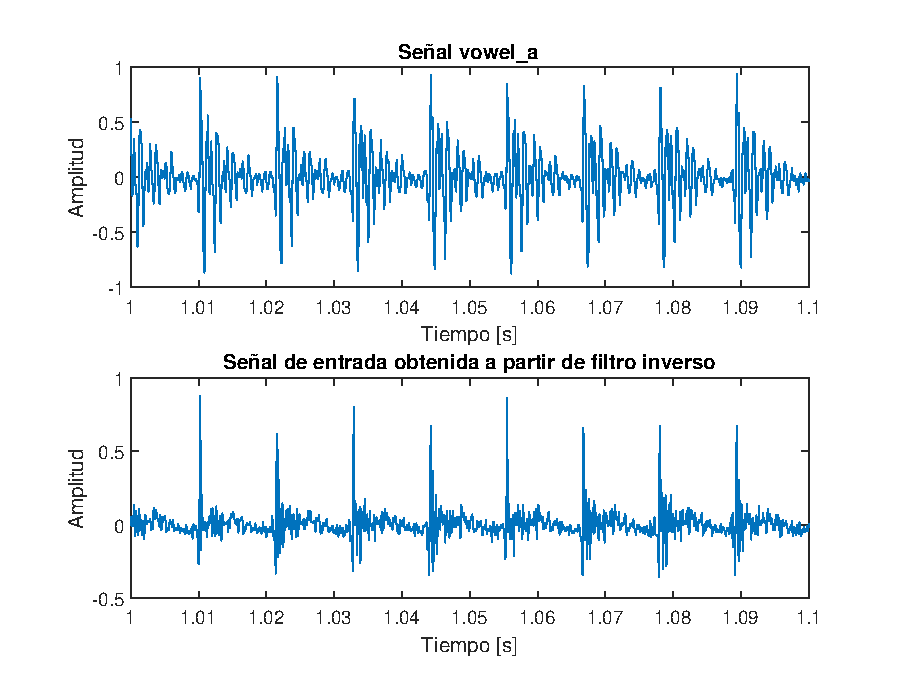
\includegraphics[width = .8\linewidth]{figures/p5_2.eps}
    \caption{Señal $vowel\_a$ y entrada $e[n]$ según filtro inverso.}
    \label{fig:p5_2}
\end{figure}

Con respecto a la forma de la señal $e[n]$ se pueden comentar que:
\begin{itemize}
    \item Modelar la entrada como un tren de impulsos para síntesis no está tan alejado de la entrada ''real'', por lo menos visualmente.
    \item La entrada tiene cierta periodicidad, por lo que se podría modelar como un tren de impulsos convolucionado con otra señal. Lo anterior puede interpretarse como que esta otra señal podría ser parte de la respuesta a impulso que el filtro AR no fue capaz de capturar (respuesta a impulso del tracto vocal). Otra interpretación sería que corresponde a la respuesta impulso de un sistema que no corresponde al del tracto vocal, como podría ser del equipo con el que se grabó o del lugar.
\end{itemize}

\subsection{Espectro en frecuencia de $e[n]$ y $vowel\_a$}

Se grafica el espectro en frecuencia de $e[n]$ y la señal $vowel\_a$, los cuales se muestran en la figura \ref{fig:p5_3}. Con respecto a los gráficos obtenidos se puede comentar que:
\begin{itemize}
    \item La señal $e[n]$ tiene un contenido en frecuencia aproximadamente plano.
    \item La respuesta en frecuencia del filtro AR de a empieza a parecer la envolvente del espectro de $vowel\_a$ debido a la naturaleza plana y ruidosa de $e[n]$. 
\end{itemize}

\begin{figure}[H]
    \centering
    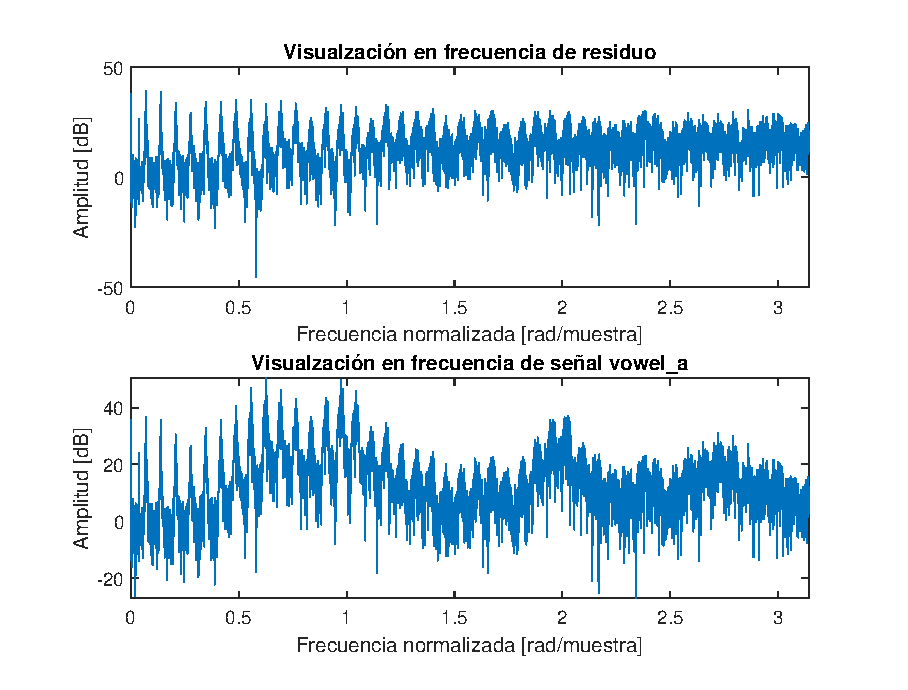
\includegraphics[width = .8\linewidth]{figures/p5_3.eps}
    \caption{Espectro en frecuencia de $e[n]$ y $vowel\_a$}
    \label{fig:p5_3}
\end{figure}

\subsection{Autocorrelación del Residuo y Frecuencia Fundamental}

Se obtiene la autocorrelación del residuo $e[n]$ y de la señal $vowel\_a$. Ambas señales se muestran en los gráficos presentes en la figura \ref{fig:p5_4}.

Para estimar la frecuencia fundamental la autocorrelación de $e[n]$ resulta bastante útil. Un peak en la autocorrelación significa que la señal tiene un gran parecido con respecto a dicho desfase de muestras, por lo que una señal que presente cierta periodicidad debiese tener peaks periódicos en su estimador de autocorrelación.

En el caso de la figura \ref{fig:p5_4}, se aprecian peaks periódicos cada un desfase $D$ aproximado de 90 muestras, por lo que la frecuencia fundamental podría estimarse como:
$$f_0 = \dfrac{1}{D\cdot T_s} =  \dfrac{1}{90\cdot (1/8000)} \approx 88.9~Hz$$

\begin{figure}[H]
    \centering
    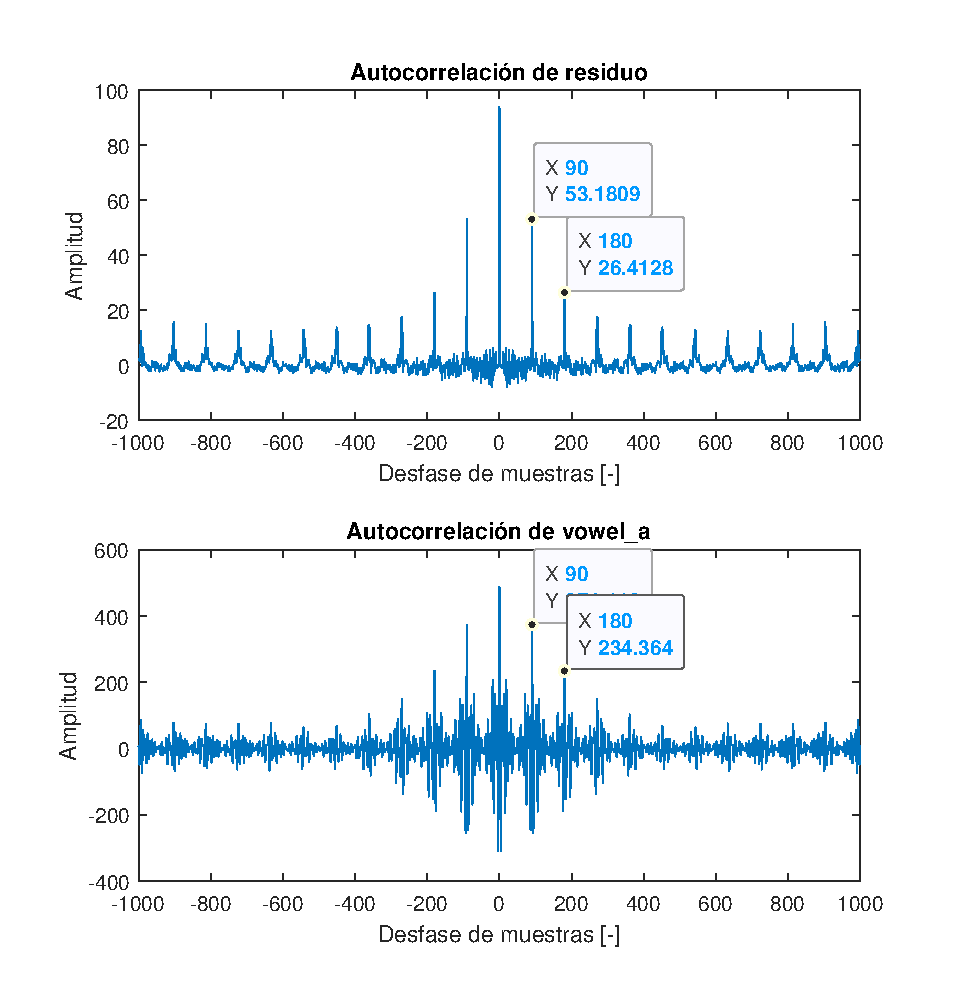
\includegraphics[width = .8\linewidth]{figures/p5_4.eps}
    \caption{Autocorrelación de $e[n]$ y $vowel\_a$}
    \label{fig:p5_4}
\end{figure}

Este método de estimación depende de que la señal este poco correlacionada en el entorno del desfase $D$ respectivo a la fundamental. De no ser así complicaría encontrar el peak, lo cual se puede apreciar levemente en la autocorrelación del la señal $vowel\_a$, ya que si bien los peaks ''importantes'' para estimar la frecuencia fundamental aún son distinguibles, un filtro de respuesta a impulso más ancha haría la tarea más complicada.
